% Preamble: Declarations & Initializations
% Defining the document class
\documentclass[a4paper, english]{report}

% Using these packages (containing macros?).
\usepackage[utf8]{inputenc}
\usepackage{csquotes}
\usepackage[backend=biber,sortcites]{biblatex}
\usepackage{Assets/DUO/duomasterforside}
\usepackage[dvipsnames]{xcolor} % for å kunne et større nummer fargemodeller i en mer fleksibel pakke
\usepackage{amsmath} % for equation*-environmentet
\usepackage{subcaption} % for subfigure-environmentet


% Considering to use:
	% \usepackage[big]{titlesec} % to customize chapters, sections, and sub-sections style in an easy way — https://www.overleaf.com/learn/latex/Sections_and_chapters
	% \usepackage{sectsty} % to customize sections, sub-sections, paragraphs, and sub-paragraphs

% Previously looked at but not found useful yet:
	% \usepackage{sidecap} % for juxtapositioning minipages next to each-other horizontally
	% \usepackage{scalerel} % for scaling objects according to references

% Setting page (configuration-) parameters.
% Headlines and Titles
\sectionfont{\fontsize{28}{34}\selectfont} % using package 'sectsty'. \fontsize{size}{baselineskip}\selectfont, where baselineskip is approx. 1.2x the size.
	
	% History Archive:
	
	% TRY 1
	% \titleformat*{\section}{\LARGE\bfseries}
	% \titleformat*{\subsection}{\large\bfseries}
	% \titleformat*{\subsubsection}{\large\bfseries}
	% \titleformat*{\paragraph}{\large\bfseries}
	% \titleformat*{\subparagraph}{\large\bfseries}
	
	% TRY 2
	% {\normalfont\Large\bfseries}{\thesection}{1em}{}
	
	% TRY 3
	% \titleformat{\section}{\normalfont\HUGE\bfseries}{\thesection}{1em}{} % using package 'titlesec'
	% \sectionfont{\LARGE} % using package 'sectsty'

% Setting new commands and functions.
% Text-editing
\newcommand{\tit}[1]{\textit{#1}}
\newcommand{\tbf}[1]{\textbf{#1}}

% Colors
\newcommand{\tcol}[2][red]{\textcolor{#1}{#2}} % default-color is red

% Page-Spacing, -Margins, and -Padding
\newcommand{\nl}{\newline}
\newcommand{\np}{\newpage}

% Lists
\newcommand{\subdash}[1]{\begin{itemize} \item{#1} \end{itemize}}

% Adding bibliography / reference-database.
\addbibresource{Assets/Bibliography/reference_database.bib}


% The Document
\begin{document}
	% Dummy chapters to get correct Chapter-numbers: (COMMENT OUT WHEN NECESSARY)
	\chapter{dummy Introduction}
	\chapter{dummy Background}
	\chapter{Baseline}
	\chapter{dummy Tools and software}
	\chapter{dummy Implementation}
	
	\chapter{Experiments and results}
	\label{chap:experiments_and_results}
	
	This chapter presents the experiments and results set up and performed in the novel synchronization simulator in Unity, as presented in Chapter \ref{chap:implementation}, for certain configurations of musical robot collectives. Effects of the individual musical robots's hyperparameters on the collective achievement and performance of achieving harmonic synchrony are presented. Some examples are hyperparameters which determines how much each musical robot will adjust itself after hearing a transmitted fire signal from a neighbouring robot; $\alpha$ for phase adjustment and $\beta$ for frequency adjustment.

	The main performance scores presented in this chapter will consist of synchronization times / simulation time (s) (i.e. how long it takes robots to reach the state of harmonic synchrony if they ever do), accompanied by the respective and corresponding error rates during the belonging simulation runs (i.e. the percentage of robot collectives out of e.g. 30 runs failing to reach harmonic synchrony before the maximum time limit of e.g. 5 minutes).

	\section{Solving the $\phi$ synchronization problem}
	This is the section where experiments attempting to solve the first and simpler problem, namely synchronizing only the phases $\phi_i$ of all agents $i$, are presented and analyzed. These are then experiments where all musical robots have an equal and fixed frequency, only adjusting phases, in order to entrain to synchronize their phases to each other until reaching harmonic synchrony.
		
		\subsection{Reproducing K. Nymoen's phase synchronization}
		In order to see that our developed synchronization simulator in Unity yields more or less the same results as K. Nymoen et al.'s firefly system \cite{nymoen_synch}, similar experiments as reported in their paper are performed. These tell us whether differences in performance, in terms of synchronization times (s), is simply due to implementation differences, or actually because of the utilized synchronization methods and hyperparameters in question. 
		
		First off, and as performed and reported in K. Nymoen et al.'s paper \cite{nymoen_synch} (c.f. their Fig. 7), Mirollo \& Strogatz's phase adjustment method (as presented in \ref{mirollo_strogatz_phase_adjust}) is experimented with for varying phase coupling constants $\alpha$, as seen in Figure \ref{fig:exp1}.
		
		\begin{figure}[ht!]
			\centering
			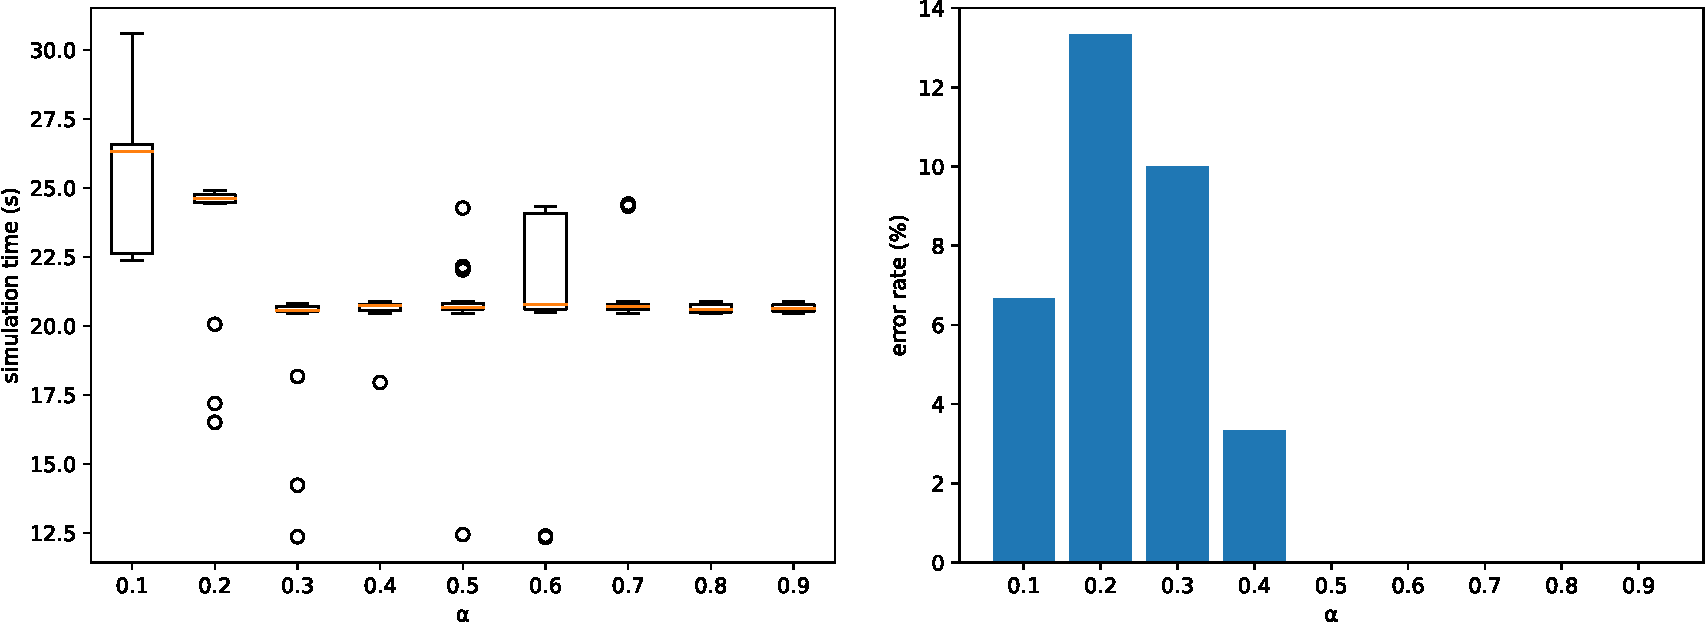
\includegraphics[width=\linewidth]{Assets/DocSegments/Chapters/ExperimentsAndResults/Figures/PerfScores/experiment1_perfScores.pdf}
			\caption{Synchronization times (s) for 6 robots with initially random and unsynchronized phases but equal and fixed frequencies (1Hz), for varying phase coupling constants $\alpha$. 30 simulation runs per $\alpha$. $\beta=0$ and $t_{ref}=50ms$. Maximum time limit was 5 minutes.}
			\label{fig:exp1}
		\end{figure}
		
		
		\subsection{Hyperparameter tuning}
		Tuning hyperparameters $\alpha$ and $t_{ref\_percentage\_of\_period}$ for several robot collective sizes, according to the performance scores of how long it takes the robot collective to achieve harmonic synchrony. Exactly these two specific hyperparameters are experimented with since they empirically seem to be the most important ones to set correctly before starting the simulator; that is, in terms of the robots actually managing to achieve harmonic synchrony.
		
		
		\subsection{Comparing phase adjustment methods}
		Now, an experiment follows where we investigate the validity of the claimed [] benefits of performing bi directional phase adjustments—both inhibitory and excitatory—compared to simply adjusting phases in an excitatory way (i.e. only ``pushing'' other ocillators's phase further or higher when firing, never ``holding'' or ``dragging'' it back).
		
		% GAMMEL EPA1-CAPTION: Performance-plot: harmonic synchronization-times from initial simulator-experiment when synchronizing phases $\phi_i$ for all agents $i$, where all phases are initially uniformly randomized between 0 and 1, and eventually synchronize and align. We here measure how long it takes 6 agents to synchronize their phases to each other, given the two different phase-adjustment methods. 30 individual runs per phase-adjustment method were performed in Unity for a collective-size of 6 agents, and $\alpha=0.2$ e.g.
		
		
		
	\section{Solving the $\phi \& \omega$ synchronization problem}
	This is the section for the experiments attempting to solve the second and harder problem of synchronizing both phases $\phi_i$, as well as frequencies $\omega_i$, for all agents $i$. These are then experiments where all musical robots originally have unequal and ever-changing phases  and frequencies, adjusting both phases and frequencies in order to entrain to synchronize their phases and frequencies until reaching harmonic synchrony.

		\subsection{Reproducing K. Nymoen's phase and frequency synchronization}
			Here we present attempts made in the novel Unity synchronization simulator at recreating K. Nymoen et al.'s first results with their novel frequency synchronization method, which is utilizing, amongst other aspects, self awareness \cite{nymoen_synch}.
			
			\paragraph{Ordering by phase couplings}
			Given that K. Nymoen et al. do not mention their $\beta$ value in their frequency synchronization experiment where they order for different phase coupling values $\alpha$, an \textit{empirically decent} $\beta$ value of 0.4 is chosen for this experiment. What \textit{empirically decent} refers to in this case are K. Nymoen et al.'s findings in the results of their last experiment \cite{nymoen_synch} where synchronization times for various $\beta$ values were evaluated; deeming $\beta=0.4$ to be a good value, with no further improvement in synchronization performance when $\beta$ is increased further. Also, when empirically observing the visual and aural signals being transmitted through the synchrony simulator in Unity, this value of $\beta=0.4$ seemed to lead to relatively stable—given original instability—simulation runs where the robot collective does manage to achieve harmonic synchrony, which is desirable when testing how fast they can synchronize.
			
			Here, K. Nymoen et al.'s self aware frequency adjustment, as implemented in the novel synchrony simulator in Unity, is experimented with for varying phase coupling constants $\alpha$ as in Figure \ref{fig:exp1} — only that this time not only phases are initially un-synchronized; robot frequencies are also initially un-synchronized. See the results in Figure \ref{fig:exp2}.
			
			\begin{figure}[ht!]
				\centering
				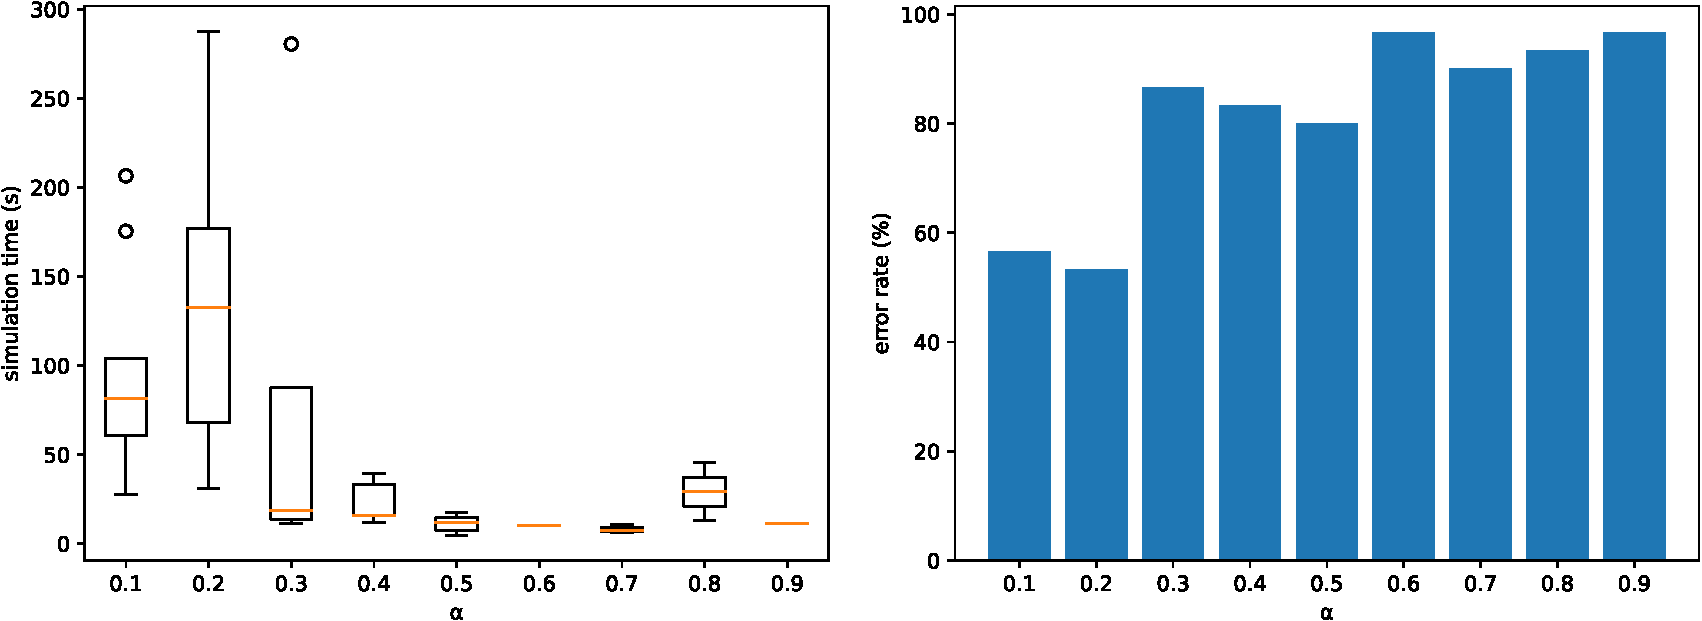
\includegraphics[width=\linewidth]{Assets/DocSegments/Chapters/ExperimentsAndResults/Figures/PerfScores/experiment2_perfScores.pdf}
				\caption{Synchronization times (s) for 6 robots with both initially random and unsynchronized phases, and frequencies, for varying phase coupling constants $\alpha$. 30 simulation runs per $\alpha$. $t_{ref}=50ms$ and $m=5$. Maximum time limit was 5 minutes.}
				\label{fig:exp2}
			\end{figure}
			
			
			\paragraph{Ordering by frequency couplings}
			
			Now, we perform the same phase \& frequency synchronization experiment as in Figure \ref{fig:exp2}, except that this time we will fix the phase coupling constant $\alpha$ and instead test how the individual musical robots's various frequency coupling constants $\beta$ affect the performance of the musical robot collective. These results are shown in Figure \ref{fig:exp3}
			
			Again, K. Nymoen et al. does not specify exactly the phase coupling constant they use in this latter experiment when testing their firefly-inspired synchronization system for various $\beta$ values. Hence, the now fixed phase coupling constant $\alpha$ is here selected by reusing the $\alpha$ value found in the similar experiment presented in Figure \ref{fig:exp2} to yield the lowest error rate in the musical robot collective when synchronizing to each other. This then gives us a fixed $\alpha = 0.2$.
			
			\begin{figure}[ht!]
				\centering
				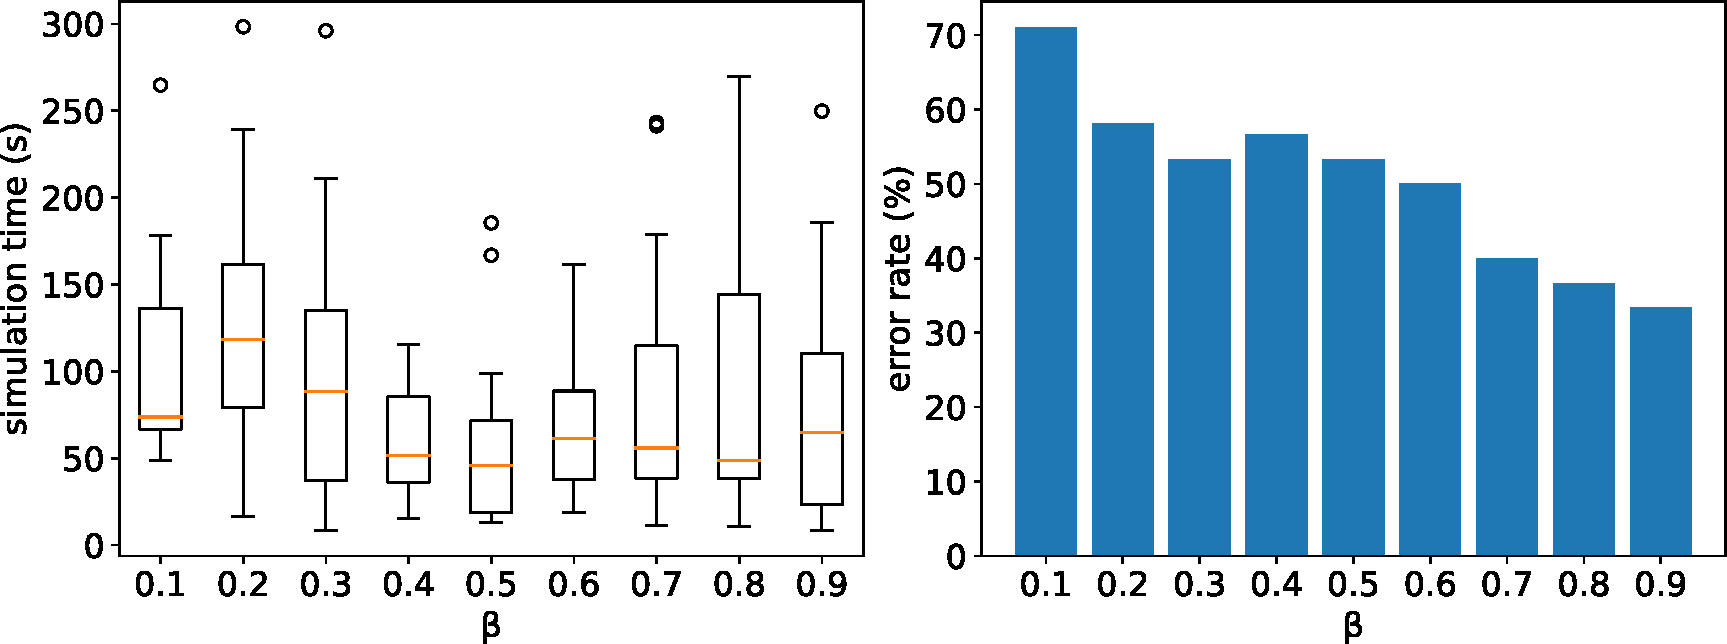
\includegraphics[width=\linewidth]{Assets/DocSegments/Chapters/ExperimentsAndResults/Figures/PerfScores/experiment3_perfScores.pdf}
				\caption{Synchronization times (s) for 6 robots with both initially random and unsynchronized phases, and frequencies, for varying frequency coupling constants $\beta$. 30 simulation runs per $\beta$. $t_{ref}=50ms$ and $m=5$. Maximum time limit was 5 minutes.}
				\label{fig:exp3}
			\end{figure}
			
			
		\subsection{Hyperparameter tuning}
		Tuning hyperparameters $\beta$ and $m$ for several robot collective sizes according to performance scores. The reason for tuning exactly these two hyperparameters, the frequency coupling constant $\beta$ and the error score list length (or memory length) $m$, is again since they seem the most significant for the synchronization performance.
		
	% Document Footer (Bibliography, Appendices etc.).
	\newpage

% Bibliography.
\printbibliography % VIL KALLE DEN 'References' ISTEDENFOR 'Bibliography'?

% Appendices (A, B, C, D, ...) {
	% A: Synonym-list w/explanations, if not managing to be consistent.
	% B: The Developed Code? Only GitHub-repo links?
	% C: Other secondary figures/plots.
% }
\end{document}